En la figura se muestra un rectángulo dividido en partes iguales. La parte sombreada representa $\frac{2}{3}$ de $\frac{3}{4}$ del rectángulo. ¿Qué fracción del rectángulo total está sombreada?

\begin{center}
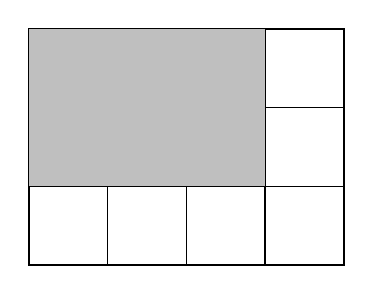
\begin{tikzpicture}
    % Dibujar rectángulo de 4x3
    \draw[thick] (0,0) rectangle (4,3);
    % Dividir en 4 columnas y 3 filas (12 cuadritos)
    \draw (1,0) -- (1,3);
    \draw (2,0) -- (2,3);
    \draw (3,0) -- (3,3);
    \draw (0,1) -- (4,1);
    \draw (0,2) -- (4,2);
    % Sombrear: 2/3 de las filas (2 de 3) y 3/4 de las columnas (3 de 4)
    % Sombreamos las 2 primeras filas y las 3 primeras columnas
    \fill[gray!50] (0,2) rectangle (3,3); % fila superior
    \fill[gray!50] (0,1) rectangle (3,2); % fila del medio
    % Nota: la fila inferior no se sombrea
\end{tikzpicture}
\end{center}